% ========================================
%	Header einbinden
% ========================================

\documentclass[bibtotoc,titlepage]{scrartcl}

% Deutsche Spracheinstellungen
\usepackage[ngerman,german]{babel, varioref}
\usepackage[T1]{fontenc}
\usepackage[utf8]{inputenc}

%\usepackage{marvosym}

\usepackage{amsfonts}
\usepackage{amssymb}
\usepackage{amsmath}
\usepackage{amscd}
\usepackage{amstext}
\usepackage{float}
\usepackage{caption}
\usepackage{wrapfig}
\usepackage{setspace}
\usepackage{threeparttable}
\usepackage{footnote}

\usepackage{caption}
\usepackage{subcaption}

\newfloat{formel}{htbp}{for}
\floatname{formel}{Formel}


\usepackage{longtable}

%\usepackage{bibgerm}

\usepackage{footnpag}

\usepackage{ifthen}                 %%% package for conditionals in TeX
\usepackage{siunitx}
%Fr textumflossene Bilder und Tablellen
%\usepackage{floatflt} - veraltet

%Fr Testzwecke aktivieren, zeigt labels und refs im Text an.
%\usepackage{showkeys}

% Abstand zwischen zwei Abs�zen nach DIN (1,5 Zeilen)
% \setlength{\parskip}{1.5ex plus0.5ex minus0.5ex}

% Einrckung am Anfang eines neuen Absatzes nach DIN (keine)
%\setlength{\parindent}{0pt}

% R�der definieren
% \setlength{\oddsidemargin}{0.3cm}
% \setlength{\textwidth}{15.6cm}

% bessere Bildunterschriften
%\usepackage[center]{caption2}


% Probleml�ungen beim Umgang mit Gleitumgebungen
\usepackage{float}

% Nummeriert bis zur Strukturstufe 3 (also <section>, <subsection> und <subsubsection>)
%\setcounter{secnumdepth}{3}

% Fhrt das Inhaltsverzeichnis bis zur Strukturstufe 3
%\setcounter{tocdepth}{3}

\usepackage{exscale}

\newenvironment{dsm} {\begin{displaymath}} {\end{displaymath}}
\newenvironment{vars} {\begin{center}\scriptsize} {\normalsize \end{center}}


\newcommand {\en} {\varepsilon_0}               % Epsilon-Null aus der Elektrodynamik
\newcommand {\lap} {\; \mathbf{\Delta}}         % Laplace-Operator
\newcommand {\R} { \mathbb{R} }                 % Menge der reellen Zahlen
\newcommand {\e} { \ \mathbf{e} }               % Eulersche Zahl
\renewcommand {\i} { \mathbf{i} }               % komplexe Zahl i
\newcommand {\N} { \mathbb{N} }                 % Menge der nat. Zahlen
\newcommand {\C} { \mathbb{C} }                 % Menge der kompl. Zahlen
\newcommand {\Z} { \mathbb{Z} }                 % Menge der kompl. Zahlen
\newcommand {\limi}[1]{\lim_{#1 \rightarrow \infty}} % Limes unendlich
\newcommand {\sumi}[1]{\sum_{#1=0}^\infty}
\newcommand {\rot} {\; \mathrm{rot} \,}         % Rotation
\newcommand {\grad} {\; \mathrm{grad} \,}       % Gradient
\newcommand {\dive} {\; \mathrm{div} \,}        % Divergenz
\newcommand {\dx} {\; \mathrm{d} }              % Differential d
\newcommand {\cotanh} {\; \mathrm{cotanh} \,}   %Cotangenshyperbolicus
\newcommand {\asinh} {\; \mathrm{areasinh} \,}  %Area-Sinus-Hyp.
\newcommand {\acosh} {\; \mathrm{areacosh} \,}  %Area-Cosinus-H.
\newcommand {\atanh} {\; \mathrm{areatanh} \,}  %Area Tangens-H.
\newcommand {\acoth} {\; \mathrm{areacoth} \,}  % Area-cotangens
\newcommand {\Sp} {\; \mathrm{Sp} \,}
\newcommand {\mbe} {\stackrel{\text{!}}{=}}     %Must Be Equal
\newcommand{\qed} { \hfill $\square$\\}
\renewcommand{\i} {\imath}
\def\captionsngerman{\def\figurename{\textbf{Abb.}}}

%%%%%%%%%%%%%%%%%%%%%%%%%%%%%%%%%%%%%%%%%%%%%%%%%%%%%%%%%%%%%%%%%%%%%%%%%%%%
% SWITCH FOR PDFLATEX or LATEX
%%%%%%%%%%%%%%%%%%%%%%%%%%%%%%%%%%%%%%%%%%%%%%%%%%%%%%%%%%%%%%%%%%%%%%%%%%%%
%%%
\ifx\pdfoutput\undefined %%%%%%%%%%%%%%%%%%%%%%%%%%%%%%%%%%%%%%%%% LATEX %%%
%%%
\usepackage[dvips]{graphicx}       %%% graphics for dvips
\DeclareGraphicsExtensions{.eps,.ps}   %%% standard extension for included graphics
\usepackage[ps2pdf]{thumbpdf}      %%% thumbnails for ps2pdf
\usepackage[ps2pdf,                %%% hyper-references for ps2pdf
bookmarks=true,%                   %%% generate bookmarks ...
bookmarksnumbered=true,%           %%% ... with numbers
hypertexnames=false,%              %%% needed for correct links to figures !!!
breaklinks=true,%                  %%% breaks lines, but links are very small
linkbordercolor={0 0 1},%          %%% blue frames around links
pdfborder={0 0 112.0}]{hyperref}%  %%% border-width of frames
%                                      will be multiplied with 0.009 by ps2pdf
%
%\hypersetup{ pdfauthor   = {Hannes Franke; Julius Tilly},
%pdftitle    = {x}, pdfsubject  = {Protokoll FP}, pdfkeywords = {V301, Innenwiderstand, Leistungsanpassung},
%pdfcreator  = {LaTeX with hyperref package}, pdfproducer = {dvips
%+ ps2pdf} }
%%%
\else %%%%%%%%%%%%%%%%%%%%%%%%%%%%%%%%%%%%%%%%%%%%%%%%%%%%%%%%%% PDFLATEX %%%
%%%
\usepackage[pdftex]{graphicx}      %%% graphics for pdfLaTeX
\DeclareGraphicsExtensions{.pdf}   %%% standard extension for included graphics
\usepackage[pdftex]{thumbpdf}      %%% thumbnails for pdflatex
\usepackage[pdftex,                %%% hyper-references for pdflatex
bookmarks=true,%                   %%% generate bookmarks ...
bookmarksnumbered=true,%           %%% ... with numbers
hypertexnames=false,%              %%% needed for correct links to figures !!!
breaklinks=true,%                  %%% break links if exceeding a single line
linkbordercolor={0 0 1},
linktocpage]{hyperref} %%% blue frames around links
%                                  %%% pdfborder={0 0 1} is the default
% \hypersetup{
% pdftitle    = {V301 Innenwiderstand und Leistungsanpassung}, 
% pdfsubject  = {Protokoll AP}, 
% pdfkeywords = {V301, Innenwiderstand, Leistungsanpassung},
% pdfsubject  = {Protokoll AP},
% pdfkeywords = {V301, Innenwiderstand, Leistungsanpassung}}
%                                  %%% pdfcreator, pdfproducer,
%                                      and CreationDate are automatically set
%                                      by pdflatex !!!
\pdfadjustspacing=1                %%% force LaTeX-like character spacing
\usepackage{epstopdf}
%
\fi %%%%%%%%%%%%%%%%%%%%%%%%%%%%%%%%%%%%%%%%%%%%%%%%%%% END OF CONDITION %%%
%%%%%%%%%%%%%%%%%%%%%%%%%%%%%%%%%%%%%%%%%%%%%%%%%%%%%%%%%%%%%%%%%%%%%%%%%%%%
% seitliche Tabellen und Abbildungen
%\usepackage{rotating}
\usepackage{ae}
\usepackage{
  array,
  booktabs,
  dcolumn
}
\makeatletter 
  \renewenvironment{figure}[1][] {% 
    \ifthenelse{\equal{#1}{}}{% 
      \@float{figure} 
    }{% 
      \@float{figure}[#1]% 
    }% 
    \centering 
  }{% 
    \end@float 
  } 
  \makeatother 


  \makeatletter 
  \renewenvironment{table}[1][] {% 
    \ifthenelse{\equal{#1}{}}{% 
      \@float{table} 
    }{% 
      \@float{table}[#1]% 
    }% 
    \centering 
  }{% 
    \end@float 
  } 
  \makeatother 
%\usepackage{listings}
%\lstloadlanguages{[Visual]Basic}
%\allowdisplaybreaks[1]
%\usepackage{hycap}
%\usepackage{fancyunits}

% ========================================
%	Angaben für das Titelblatt
% ========================================

\title{Lehrstuhlversuch E1 - Röntgenreflektometrie\\				% Titel des Versuchs 
\large TU Dortmund, Fakultät Physik\\ 
\normalsize Fortgeschrittenen-Praktikum}

\author{Jan Adam\\			% Name Praktikumspartner A
{\small \href{jan.adam@tu-dortmund.de}{jan.adam@tu-dortmund.de}}	% Erzeugt interaktiven einen Link
\and						% um einen weiteren Author hinzuzfügen
Dimitrios Skodras\\					% Name Praktikumspartner B
{\small \href{dimitrios.skodras@tu-dortmund.de}{dimitrios.skodras@tu-dortmund.de}}		% Erzeugt interaktiven einen Link
}
\date{09.06.2015}				% Das Datum der Versuchsdurchführung

% ========================================
%	Das Dokument beginnt
% ========================================

\begin{document}

% ========================================
%	Titelblatt erzeugen
% ========================================

\maketitle					% Jetzt wird die Titelseite erzeugt
\thispagestyle{empty} 				% Weder Kopfzeile noch Fußzeile

% ========================================
%	Der Vorspann
% ========================================

%\newpage					% Wenn Verzeichnisse auf einer neuen Seite beginnen sollen
%\pagestyle{empty}				% Weder Kopf- noch Fußzeile für Verzeichnisse

\tableofcontents

%\newpage					% eine neue Seite
%\thispagestyle{empty}				% Weder Kopf- noch Fußzeile für Verzeichnisse
%\listoffigures					% Abbildungsverzeichnis

%\newpage					% eine neue Seite
%\thispagestyle{empty}				% Weder Kopf- noch Fußzeile für Verzeichnisse
%\listoftables					% Tabellenverzeichnis
\newpage					% eine neue Seite


% ========================================
%	Kapitel
% ========================================

%\section{Einleitung}				% Bei Bedarf

\section{Theorie}
\subsection{Fresnelsche Formeln}
Die Fresnelformeln geben den Reflexions- (R) und den Transmissionsgrad (T) von EM-Wellen an der Grenzfläche zweier Medien mit Brechungsindizes $n_1$ und $n_2$ an.
Entsprechend der beiden Polarisationsrichtungen (senkrecht und parallel) gibt es vier verschiedene Formeln
\begin{align}
 T_s &= \frac{2n_1}{n_1 \cos\alpha + n_2\cos\beta}\\
 R_s &= \frac{n_1 \cos\alpha - n_2\cos\beta}{n_1 \cos\alpha + n_2\cos\beta}\\
 T_p &= \frac{2n_1}{n_2 \cos\alpha + n_1\cos\beta}\\
 R_p &= \frac{n_2 \cos\alpha - n_1\cos\beta}{n_2 \cos\alpha + n_1\cos\beta},
\end{align}
\noindent mit $\alpha$ als Winkel zwischen einfallendem Strahl und Lot und $\beta$ als Winkel zwischen ausfallendem Strahl und Lot. Das Lorentz-Modell erklärt,
dass Materie für Röntgenstrahlung einen Brechungsindex $n = 1-\delta <1$ aufweist. Hierin lautet die dielektrische Funktion
\begin{align}
 \epsilon(\omega) = 1 + \frac{4\pi n_0 e^2}{m_\text{e}} \sum\limits_i \frac{f_i}{\omega_i^2 - \omega^2 - \text{i}\omega\Gamma_i},
\end{align}
für Materialien mit $Z=\sum_i f_i$ Elektronen pro Atom mit $i$ unterschiedlichen Eigenfrequenzen $\omega_i$ und Dämpfungen $\Gamma_i$. $n$ erhält man als
Realteil von $\sqrt{\epsilon}$ und lautet $f_i / \omega_i^2 - \omega^2$. Dieser wird für Röntgenstrahlung ($\omega_i <\omega$) negativ und $n<1$, was
unterhalb eines kritischen Winkels $\alpha_c$ an der Grenzfläche zur Totalreflexion führt. Die Abweichung $\delta$ ist vernachlässigbar, sodass 
$n_1 \approx n_2 \approx 1$ genähert wird und Polarisationen nicht mehr unterschieden werden. Hiermit wird die Gesamtreflektivität $R_F = |R_{s,p}|^2$ für
große Winkel zu
\begin{align}
 R_F \approx \left(\frac{\alpha_c}{\alpha_i}\right)^2.
\end{align}

\subsection{Zweischichtsystem}
Kiessing-Ringe sind Modulationen der Reflexionskurve, hervorgerufen durch Interferenz der reflektierten Strahlung. Die Minima entstehen, wenn der 
Phasenunterschied gerade ein ungerades Vielfaches der Wellenlänge $\lambda$ ist. Ziel hier ist eine Beziehung zwischen der Winkeldifferenz zweier Kiessing-Minima 
in Beziehung zur Schichtdicke $d$ zu setzen. Der Gangunterschied liest sich
\begin{align}
 \delta = 2 d \sin\alpha.
\end{align}
Die Gangunterschieddifferenz ist daher
\begin{align}
 \delta_n -\delta_{n-1}= 2 d \sin\alpha_n - 2d\sin\alpha_{n-1}.
\end{align}
Die linke Seite entspricht je ungeradzahligen Vielfachen der Wellenlänge. Weiterhin kann man kleine Winkel annehmen $\sin\alpha \approx \alpha$, was zur
gesuchten Relation führt
\begin{align}
 d \approx \frac{\lambda}{2\Delta\alpha_i} = \frac{2\pi}{\Delta q_z}
\end{align}

\subsection{Parratt-Algorithmus}
Bei mehreren Schichten wird die Reflektivität durch Überlagerung unterschiedlicher Brechungsindizes komplizierter. Hierzu wird der Paratt-Algorithmus als
rekursive Lösung verwandt. Mit $r_{j,j+1} = \frac{k_{z,j}-k_{z,j+1}}{k_{z,j}+k_{z,j+1}}$ an Grenzfläche $j$ und $z$-Komponente $k_{z,j} = k\sqrt{n_j^2-\cos^2\alpha_i}$
lautet das Amplitudenverhältnis nach dem Algorithmus
\begin{align}
 X_j = \frac{R_j}{T_j} = \text{e}^{-2ik_{z,j}z_j}\frac{r_{j,j+1} + X_{j+1} \text{e}^{+2ik_{z,j}z_j}}{1 + r_{j,j+1} X_{j+1}\text{e}^{+2ik_{z,j}z_j}}.
\end{align}
Angewandt auf ein System mit $N=2$ Schichten mit unendlich dicken Vakuum und Substrat. Somit gilt als Startwert $X_3 = 0$ und damit für die beiden weiteren
\begin{align}
 X_2 &= r_{2,3}\text{e}^{-2ik_{z,2}z_2}\\
 X_1 &= \frac{r_{1,2}+\text{e}^{-2ik_{z,2}z_2}}{1+r_{1,2}\text{e}^{-2ik_{z,2}z_2}}.
\end{align}
Mit \texttt{Python} lässt sich die Reflektivität graphisch (Abbildung \ref{pic_ReflNormal}) darstellen.

\begin{figure}[H]
 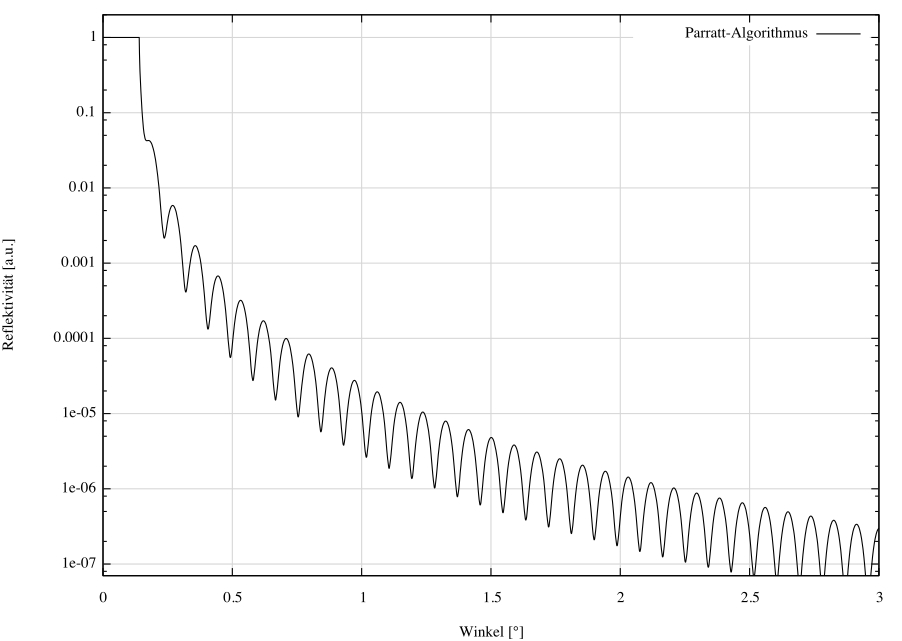
\includegraphics[width=\textwidth]{../pics/normal.jpg}
 \caption{Reflektivität mit dünner Schicht ($500$ $\mathring{A}$) und unendlich dickem Substrat, ermittelt durch den Parratt-Algorithmus}
 \label{pic_ReflNormal}
\end{figure}
\noindent
Erweitern lässt sich dieses System noch um die Rauigkeit $\sigma$, was zu den modifizierten Fresnelformeln führt
\begin{align}
 r^\sigma_{j,j+1} = r_{j,j+1} \cdot \text{e}^(-2k_{z,j}k_{z,j+1}\sigma_j^2.
\end{align}
Mit einem $\sigma = 6\mathring{A}$ und sonst identischen Parametern verändert sich die Kurve so, wie in Abbildung \ref{pic_ReflRau} gezeigt. Die Kurve fällt aufgrund
der Rauigkeit deutlich schneller ab.

\begin{figure}[H]
 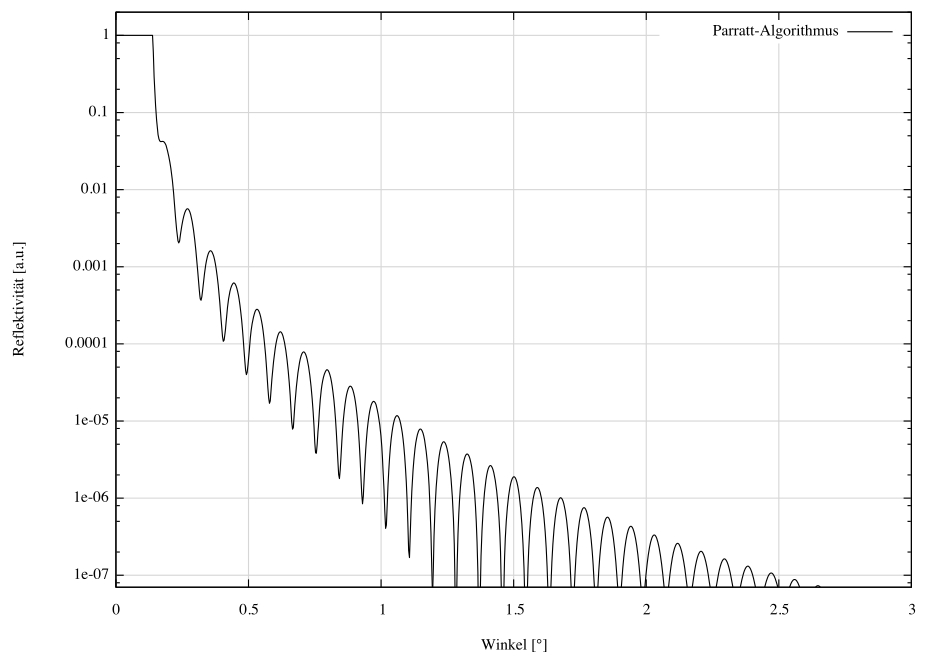
\includegraphics[width=\textwidth]{../pics/rau.jpg}
 \caption{Reflektivität mit dünner Schicht ($500$ $\mathring{A}$) und unendlich dickem Substrat, ermittelt durch den Parratt-Algorithmus. Die Rauigkeit des Substrats ist berücksichtigt}
 \label{pic_ReflRau}
\end{figure}


\section{Durchführung}
Bei der Durchführung des Versuchs müssen zu Beginn Strahl und Probe justiert werden. Dazu werden folgende Schritte getätigt:
\begin{enumerate}
 \item Die Probe wird in das Labordiffraktometer eingeführt.
 \item Die Probe wird entlang der $z$-Achse aus dem Strahlengang gefahren.
 \item Der Detektor wird zur Röntgenröhre ausgerichtet. (Detektor Scan)
 \item Die $z$-Koordinate der Probe wird so gewählt, dass die dann gemessene Intensität gerade der halben Maximalintensität entspricht. (z-Scan)
 \item Der Strahlengang wird parallel zur Probenoberfläche eingestellt. (Rocking Scan)
 \item Die $z$-Koordinate der Probe wird erneut so gewählt, dass die dann gemessene Intensität der halben Maximalintensität entspricht. (z-Scan)
 \item Die Detektorröhre wird so eingestellt, dass sie bei Totalreflexion ($15^\circ$) genau im reflektierten Strahl liegt. (Rocking Scan)
 \item Die $z$-Koordinate der Probe wird erneut so gewählt, dass die dann gemessene Intensität der halben Maximalintensität entspricht. (z-Scan)
 \item Für große Einfallswinkel muss nun noch eine Feinjustage des Detektors folgen. Dazu wird ein Rocking Scan um $2\theta=1^\circ$ durchgeführt, also einem
 Winkelbereich von ca. 0.45 bis 0.55 und der Detektorwinkel wird auf 0.5 geeicht.
\end{enumerate}
Nach Justage des Labordiffraktometers kann nun mit der Vermessung der Probe begonnen werden. Als Scanbereich (Winkel) wird das Intervall $0^\circ$ bis 
$2.5^\circ$ mit einer Schrittweite von $0.0025^\circ$ gewählt. Pro Winkel wird die Intensität über eine Zeitraum von $t=\SI{10}{\second}$ gemessen. Um Fehler durch
Streustrahlen zu vermindern, wird außerdem ein ``Diffuser Scan'' durchgeführt. Dabei wird die eben beschriebene Messung wiederholt, jedoch mit einem um
$0.1^\circ$ verschobenen Detektor.

\section{Auswertung}
In diesem Versuch sollen Dispersion und Rauigkeit des Siliziumwafers, sowie die Schichtdicke, Dispersion und Rauigkeit der Polysterolschicht bestimmt werden.

\begin{figure}[h]
	\centering
	\includegraphics[width=\textwidth]{../tex/bilder/data.pdf}
	\caption{Messwerte des Reflektivitätsscans und des diffusen Scans.}
	\label{pic:daten}
\end{figure}

Abbildung \ref{pic:daten} zeigt die beim Scan aufgenommenen Daten. Nach der eigentlichen Reflektivitätsmessung wurde ein sogenannter "Diffuser Scan"\ durchgeführt, bei dem der Detektorwinkel um \SI{0.1}{\degree} gegenüber dem Einfallswinkel verschoben wurde. Dadurch wird der Anteil des gestreuten Röntgenlichts gemessen welches vom Reflektivitätsscan abgezogen werden muss.

Anschließend müssen die Daten um den Geometriefaktor $G$ korrigiert werden.
Der Geometriefaktor entspricht dem Anteil des Strahls, der die Fläche des Wafers trifft:
\begin{align}
	G &= \frac{D}{d_0}\cdot \sin(\alpha_i) &\text{für $\alpha_i < \alpha_g$}\\
	G &= 1 &\text{sonst}
\end{align}
 und somit in Richtung des Detektors reflektiert wird. Bei Winkeln $\alpha_i >$ Geometriewinkel $\alpha_g$, trifft immer der gesamte Strahl auf die Probe, daher gilt dort $G=1$. Bei kleineren Winkeln geht jedoch ein Teil des Lichts verloren, wodurch nur ein Teil des eigentlichen Signals im Detektor gemessen wird. Hier muss das Signal um den Geometriefaktor korrigiert werden.

Bei einem Strahldurchmesser von $D = \SI{0.1}{\milli\meter}$ und einer Probendicke von $d_0 = \SI{30}{\milli\meter}$ ergibt sich für den Geometriewinkel $\alpha_g$ ein Wert von
\begin{align}
	\alpha_\text{g} = \arcsin\left(\frac{d_0}{D}\right) = \SI{0.191}{\degree}.
\end{align}
Unterhalb dieses Winkels muss der Geometriefaktor bei der Auswertung berücksichtigt werden. In Abbildung \ref{pic:geometrie} sind sowohl die ursprüngliche Datenreihe, als auch die korrigierte Datenreihe eingetragen. Bei kleinen Winkeln beträgt die Korrektur mehr als eine Größenordnung.

\begin{figure}[h]
	\centering
	\includegraphics[width=\textwidth]{../tex/bilder/geometriefaktor.pdf}
	\caption{Messwerte mit und ohne Korrektur durch den Geometriefaktor.}
	\label{pic:geometrie}
\end{figure}


Um nun Dispersion und Rauigkeit des Siliziumwafers, sowie Schichtdicke, Dispersion und Rauigkeit der Polysterolschicht zu bestimmen, wird mittels Python ein Fit der aufgenommenen Messwerte durchgeführt. Der Brechungsindex der Luft wird dabei konstant als $n_1=1$ angenommen.

In Abbildung \ref{pic:fit} wurde neben den Datenpunkten zwei gefittete Kurven eingetragen. Die blaue Kurve ergibt sich durch die Parameter, die das Pythonscript errechnet hat:
\begin{align*}
	n_2 &= 1-2.8\cdot 10^{-6}\\
	n_3 &= 1-7.2\cdot 10^{-6}\\
	\sigma_1 &= 5.5\cdot 10^{-10} \\
	\sigma_2 &= 2.4\cdot 10^{-10}\\
	z_2&= 210.0\cdot 10^{-10}
\end{align*}

Die blaue Kurve weicht jedoch um bis zu 30\% von den Messwerten ab. Daher wurden die angegebenen Parameter per Hand weiter optimiert, um eine bessere Abdeckung zu erzielen. Die neue Kurve wird in rot dargestellt.
\begin{figure}[h]
	\centering
	\includegraphics[width=\textwidth]{../tex/bilder/fit.pdf}
	\caption{Messwerte mit und ohne Korrektur durch den Geometriefaktor}
	\label{pic:fit}
\end{figure}


Die rote Kurve ergibt sich durch folgende Parameterwahl:
\begin{align*}
n_2 &= 1-3.5\cdot 10^{-6}\\
n_3 &= 1-9.24\cdot 10^{-6}\\
\sigma_1 &= 4.78\cdot 10^{-10} \\
\sigma_2 &= 3.28\cdot 10^{-10}\\
 z_2&= 209.8\cdot 10^{-10}
\end{align*}

\section{Diskussion}
Es gelingt nicht, eine perfekte Übereinstimmung zwischen Messwerten und Theoriekurve zu erzielen.
Dies deutet darauf hin, dass die Struktur der untersuchte Probe vom Theoriemodell abweicht. In der Tat bildet sich durch den Sauerstoff aus der Luft auf der Siliziumschicht eine feine Oxidschicht, die im verwendeten Modell nicht berücksichtigt wurde.
Entsprechend gelingt es dem automatischen Fit nicht, die bestmöglichste Übereinstimmung zu finden.

Durch eine manuelle Optimierung kann die Theoriekurve den Messwerten weiter angenähert werden, eine sehr gute Übereinstimmung kann jedoch entweder nur im ersten Peak oder nur in den nachfolgenden Erreicht werden. Hier wurde ein Tradeoff aus beidem gewählt, um starke lokale Schwankungen zu vermeiden.

Beide Auswertungen gelangen zu einer ähnlichen Schichtdicke des Siliziums von etwa \SI{210}{\angstrom}.
Die Rauigkeit dieser Schicht variiert jedoch je nach Fit zwischen \SI{2.4}{\angstrom} und \SI{3.2}{\angstrom}, was ein Hinweis auf die vorhandene Oxidschicht sein kann.



\vspace{2cm}
\textbf{Literatur}

\vspace{0.3cm}
[1] Anleitung des Lehrstuhlversuchs

% ========================================
%	Literaturverzeichnis
% ========================================

%\bibliographystyle{plainnat}			% Bibliographie-Style auswählen
%\bibliography{BIBDATEI}			% Literaturverzeichnis

% ========================================
%	Das Dokument endent
% ========================================

\end{document}
